\chapter{计算机病毒的治愈}

如果需要广泛共享,预防计算机病毒可能是不可行的,与生物学的类比让我们看到了可以用一种保护的方式来进行治愈。治愈在生物系统取决于检测病毒的能力,并且要找到一种方法来克服它。类似的可用于计算机病毒。我们现在测试计算机病毒的检测和清除的能力。

\section{病毒的检测}

为了确定一个给定的程序‘P’是一种病毒,必须确定P可以感染其他程序。这是不可判定的,因为P可以调用决策过程‘D’并感染其他程序当且仅当D确定P不是病毒。我们得出这样的结论,一个程序通过检查其外观精确的将病毒从其他程序区分开来是不可行。在接下来对程序V的修
改中
(图\ref{fig6}),
我们假设决策
过程D返回“真”当且仅当其参
数是一个病毒,
这是病毒检测的不可判定性的例证。


\begin{figure}[h!]
    \centering
    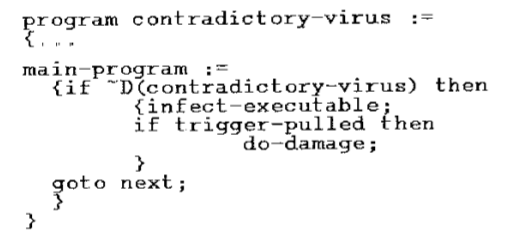
\includegraphics[width=0.60\textwidth]{figure/fig6.png}
    \caption{Contradiction of a virus C} 
    \label{fig6}
\end{figure} 
通过修改V的主要程序,我们可以保证,如果决策过程D决定CV是一个病毒,CV不会感染其他程序,因此不会表现为一个病毒。如果D确定CV不是病毒,CV会传染给其他程序,因此成为一个病毒。因此,假设决策过程D是自我矛盾的,从外观精确检测病毒是不可判定的。


\section{病毒的演化}

在我们的实验中,一些病毒花了不到4000个字节通用计算机上实现。由于我们可以交错任何不终止的程序,在有限时间内终止并且不复写病毒或其状态变量,并仍有病毒,那么一个单一病毒可能变异的数量显然是非常大的。在这个例子中考虑演化的病毒EV,我们通过允许它在任何两个必要的声明间添加随机语句来增加V。

一般来说,程序的‘P’的两个演化(‘P1’和‘P2’)的等价性证明是不可判定的,这是因为任何决策过程‘D’都可以调用P1和P2找到他们的等价。如果发现等价的他们执行不同的操作,并且发现不同的他们的行为相同,因此是等价的。图8显示对程序EV修改,决策过程D返回“真”当且仅当两个输入程序是等价的。
程序UEV会演变成P1和P2两种类型的
程序之一。如果程序类型是P1,状态标记“zzz”将成为:


如果D(P1,P2),打印1;

而如果程序类型是P2,状态标记“zzz”将成为:

如果D(P1,P2),打印0;

\begin{figure}[h!]
    \centering
    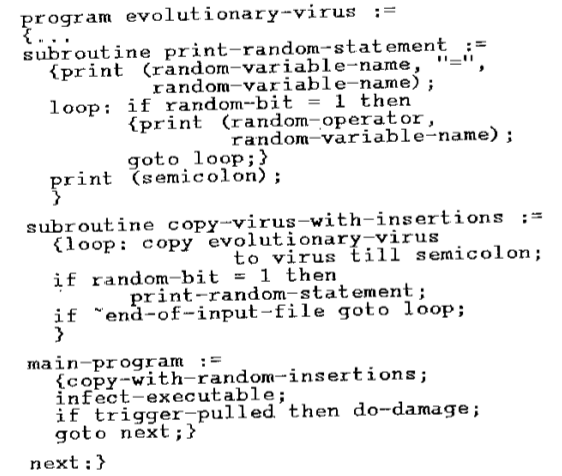
\includegraphics[width=0.60\textwidth]{figure/fig7.png}
    \caption{Evolutionary virus EV} 
    \label{fig7}
\end{figure} 

两个演化分别调用决策过程D来决定他们是否是等价的。如果D表明他们是等价的,那么P1将打印1而P2将打印一个0,并且D会矛盾。如果D表明他们是不同的,就不打印任何东西。否则它们是平等的,D再次矛盾。因此,假设决策过程D是自我矛盾的,并且通过外表精确的确定这两个程序的等价性不可判定的。

因为P1和P2是相同的程序的演化,程序演化的等价性是不可判定的,并且因为他们都是病毒,所以病毒演化的等价性也是不可判定的。程序UEV还演示了这两种非等价的演化都可以病毒。

\begin{figure}[h!]
    \centering
    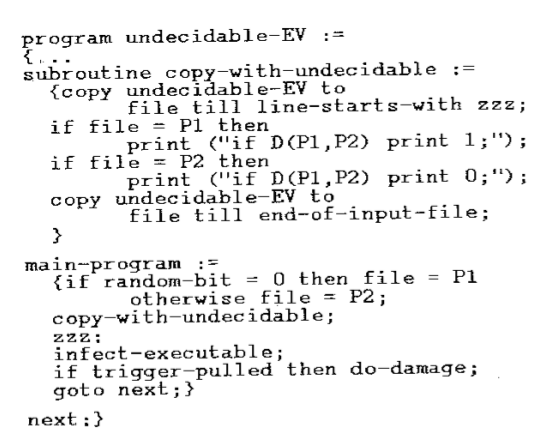
\includegraphics[width=0.60\textwidth]{figure/fig8.png}
    \caption{Undecidable equivalence of evolution of a virus UEV} 
    \label{fig8}
\end{figure} 

另一种外观检测的方法,是从行为进行检测。病毒,就像任何其他的程序,为用户请求服务时作为一个代理,并且使用的病毒进行合法的使用时是合法的。行为检测问题成为一个定义,定义系统服务的使用是否合法,并找到一种检测的方法。

作为一个合法的病毒的例子,一个编译器编译的新版本实际上是本身,根据这里的定义它也是一种病毒。这是一个程序,通过修改它本身到一个进化版去感染另一个程序。由于病毒的能力在大多数编译器中存在,每一次编译器的使用就是一个潜在的病毒攻击。编译器的病毒活动仅仅是由特定的输入触发,从而为了检测触发,必须能够从外表检测病毒。由于通过行为精确检测导致通过外表精确检测输入,并且由于通过外表精确检测是不可判定的,由此可见,通过行为精确检测的行为也不可判定的。

\section{有限的病毒防护}

病毒的一个有限形式已经通过一个特殊版本的C编译
器设计出来了\upcite{24},可以检测登
录程序的编译,并添加一个木马,让作者登
录。因此作者可以通过这个编译器访问
任何Unix系统。此外,新版本的编译器
可以检测到编译本身的演化版本,并让
他们感染同样的木马。


作为对策,我们可以设计一个新的登录程序(和C编译器)充分不同于原始以使得等价性很难确定。如果“当今最好的人工智能程序”在给定的时间内无法检测等价性,并且编译器执行其任务不需要那么多时间,此时它可以合理假设病毒不可能检测到等价性,并且不会传播给自身。如果检测的确切性质是已知的,它可能是很简单的工作。一旦一个病毒自由的编译器产生,老版本可以被重新编译以便于进一步的应用。



虽然我们已经表明,一般情况下是不可能检测到病毒的,但是任何特定的病毒可以由一个特定的检测方案进行检测。例如,病毒V可以通过寻找1234567作为可执行文件的第一行来很容易地探测到。如果这个可执行文件被感染了,它就无法运行,也就无法传播了。
使用图\ref{fig9}中的程序代替正常运行的命令,
并拒绝可执行程序感染病毒V。


\begin{figure}[h!]
    \centering
    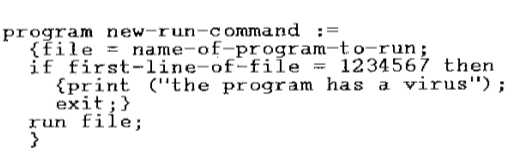
\includegraphics[width=0.60\textwidth]{figure/fig9.png}
    \caption{Protection from virus V} 
    \label{fig9}
\end{figure} 


同样,任何特定的检测方案可以由一个特定
的病毒规避。作为例子,如果攻击者知
道用户使用程序PV免受病毒的攻击,病毒V 可以很
容易地替换为V’,即把第一行1234567
改为123456。更复杂的防御方案和病毒可以进行测
试。显然,不能检测到的感染不存在,
不被感染的检测机制不存在。


这个结果导致病毒和防御可能平衡地存在,因此一个给定的病毒只能损害一个系统指定的一部分,而一个给定的防护方案只能预防给定的一组病毒。如果每个用户和攻击者使用相同的防御和病毒,会有一个最终的病毒或防御。从攻击者的观点和防卫者的观点(可能不兼容)有一组病毒和防御是有意义的。


在病毒和防护方案不进化的情形下,这可能会产生某
些固定的幸存者,但是那些可以进化为难以
攻击的程序(或者病毒)的部分可以更容易存
活。随着演化的发生,平衡倾向于改变,但最简单的
情况下最终的结果也是不清楚的。这是生物
进化理论\upcite{6}的一个重要的类比,并可能与疾病
的遗传理论相关。同样,病毒通过系统的
传播可以通过对传染病的研究来建立数学模型\upcite{2}。


由于我们无法精确的检测病毒,我们剩下的问题是用一种决定性的容易计算的方式来定义潜在的非法使用方式。我们可能愿意检测很多不是病毒的程序,甚至为了检测大量的病毒而不检测一部分的病毒。如果一个事件是相对罕见的“正常”使用,那么它具有较高的信息内容,并且我们可以定义一个报告完成时的阈值。如果有足够的仪器可用,流列表可以保持跟踪所有用户影响道德任何给定的文件。那些出现在许多来流列表中的用户可以被认为是可疑的。用户输入流列表的速率也可以作为病毒检测的良好指标。

如果病毒很少被其他程序使用,那么这种类型的测量是有价值的,但是也有几个问题。如果攻击者知道阈值,那么病毒仍然可以工作。一个智能阈值方案可以使得阈值不容易被攻击者决定。尽管这种“游戏”可以来回进行,但是可能使得感染频率足够低缓慢而未被检测的病毒无法合法使用。

检查了几个系统防御病毒攻击的能力。令人惊讶的是,这些系统包括程序的所有者都不能被其他用户使用。作这类标记必须几乎肯定会使得用最简单的病毒攻击都能被检测到。

一旦病毒植入,它可能不容易被完全删除。如果在删除的同时系统保持运行,消毒程序可能会再次感染。这展现了一个无限的尾巴追逐的过程。没有一些拒绝服务的存在,删除是不可能的,除非程序执行删除的速度比病毒传播的速度快。即使在移除是慢于病毒感染速度的情况,它可能会允许大多数活动在删除过程中继续进行,不需要删除的过程很快。例如,可以隔离用户中的一个或者一群,并且治愈他们而不用拒绝其他用户的服务。

一般来说,精确的删除取决于精确的检测,因为如果没有精确的检测,不可能精确的指导给定对象是否要删除。在特殊情况下,它可能会用一个不精确的算法执行删除过程。作为例子,每个写在给定的日期后的文件可以被删除,以便于删除任何从那个日期开始之后的病毒。如果在病毒攻击之前有很长的休眠期,那么这种方法非常有破坏性,因为在清理系统的过程中就算是备份也要被移除。

一个担心在上面已经表达了,另一个是容易休眠是病毒自发产生的机会。一个密切相关的问题是N个猴子在N个键盘上需要多长的时间来创建一个病毒,这和休眠有着类似的调度。


